\chapter{ESTADO DA ARTE}\label{sec:cap3}

%\resumodocapitulo{resumo del capitulo}
\vspace{1cm}
Desde que o homem descobriu como usar estímulos elétricos para melhorar a dor ou gerar contrações musculares artificialmente foram desenvolvidos métodos de eletroestimulação baseados inicialmente em animais (e.g. arraia elétrica \cite{Heidland2013NeuromuscularWaisting}) que geravam choques elétricos até dispositivos eletromédicos chamados de eletroestimuladores. 

Os eletroestimuladores de uso comum normalmente aplicam o estímulo elétrico com eletrodos superficiais, isto por sua facilidade de colocação e uso. Também, o estímulo elétrico pode ser aplicado ao tecido neural e/ou músculo por meio de eletrodos implantados ou percutâneos. Dentro dos dispositivos de estimulação elétrica estão os disponíveis comercialmente e os de pesquisa. Estes aparelhos podem se encontrar nas mais diversos ambientes e aplicações: dispositivos de auxílio na marcha (como pé caído), dispositivos para o fortalecimento dos músculos, dispositivos de estimulação de órgãos como bexiga, coração, entre muitos outros.

Nesse contexto, neste capitulo é feita uma revisão da literatura iniciando com uma perspectiva histórica do início dos aparelhos de eletroestimulação, seguidos pelos sistemas contemporâneos de eletroestimulação descritos na literatura científica e finalmente os dispositivos disponíveis comercialmente. O foco aqui se dá nos dispositivos envolvendo estimulação com eletrodos superficiais.


\section{PERSPECTIVA HISTÓRICA}

Em 1768 foram desenvolvidos os primeiros eletroestimuladores. Estes dispositivos eram máquinas de diferentes formas que produziam eletricidade estática. Existiram muitos tipos de máquinas eletroestáticas, mas a mais comum foi a máquina formada por um disco rotativo como mostrado na Figura \ref{fig:ma_f1} \cite{Geddes1994TheBiology}. Em 1791 Galvani usou uma máquina eletrostática de disco rotativo que o permitiu descobrir e estudar a bioeletricidade.

%figura c3_1
\begin{figure*}
    \centering %
    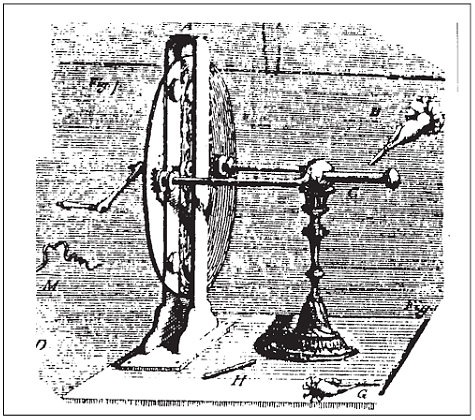
\includegraphics[width=0.4\linewidth]{figs/Fig_c3/ma_f1}
    \caption{Eletroestimulador baseado em máquina de eletricidade estática \cite{Geddes1994TheBiology}.}
    \label{fig:ma_f1}
\end{figure*}

Outros eletroestimuladores foram desenvolvidos com o tempo, como o eletroestimulador com capacitores chamado de \textit{Leyden jar} usados para propósitos de entretenimento \cite{Geddes1994TheBiology}. Em seguida foram desenvolvidas células eletroquímicas que produziam corrente. Essas células foram conectadas a um interruptor, fazendo possível iniciar e parar a corrente. Com o tempo os interruptores foram melhorados permitindo o controle da repetição e duração da corrente. Consequentemente estes tipos de dispositivos foram chamados de \textit{Rheotomes}, que remete à ideia de “cortador de fluxo” \cite{Geddes1994TheBiology}. Não obstante, com o descobrimento da indução magnética por Michael Faraday em 1831, uma nova forma controle de corrente permitiu o desenvolvimento de um novo tipo de eletroestimulador. Este tipo de dispositivo foi chamado \textit{Inductorium} \cite{Geddes1994TheBiology}.

O \textit{Leyden jar}, o \textit{Rheotomes} e o \textit{Inductorium} permitiram criar as bases da eletroterapia. No entanto eram dispositivos rudimentares que não ofereciam condições suficientes para melhorar o entendimento da corrente elétrica como agente terapêutico. Nesse contexto, os eletroestimuladores modernos foram desenvolvidos somente depois da segunda guerra mundial, trazendo grandes contribuições no estudo da aplicação de estimulação elétrica \cite{Faria2006ImplementacaoMedulares}. 

Albert Grass em 1940 desenvolveu um dos primeiros eletroestimuladores para uso em pesquisa (ver Figura \ref{fig:pes_f2}), um sistema que permitia controlar de forma independente a frequência e a largura do pulso \cite{Geddes1994TheBiology}. A partir daí e mais precisamente entre os anos 1952 e 1965, foram construídos equipamentos de eletroestimulação para diferentes fins, como o marca-passo ou uso da estimulação para a modulação da dor \cite{Faria2006ImplementacaoMedulares}.  

% Figura c3_2
\begin{figure*}
    \centering %
    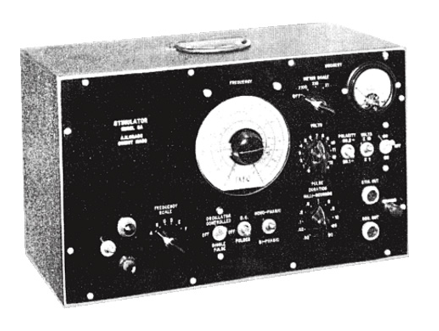
\includegraphics[width=0.4\linewidth]{figs/Fig_c3/pes_f2}
    \caption{Um dos primeiros eletroestimuladores desenvolvido para pesquisa \cite{Geddes1994TheBiology}.}
    \label{fig:pes_f2}
\end{figure*}


Depois, nos anos 70, a estimulação elétrica avançou bastante. Equipamentos para estimulação foram desenvolvidos para aplicações no esporte, como foi na União Soviética com o Dr. Yacov Kots, que se interessou pela primeira vez no desenvolvimento da força nos esportistas usando estimulação elétrica \cite{Cometti2007BibliografiaElectroestimulacion}. No seu estudo, Kots usou estimulação para aumentar a força muscular na Contração Voluntária Máxima (\acrshort{CVM}) dos atletas de elite soviéticos, o que resultou numa melhoria no seu rendimento esportivo.

Outros autores na Itália, Canadá, Polônia e Estados Unidos entre os anos 1970 a 1981 desenvolveram estudos sobre a estimulação elétrica aplicada ao esporte, nos quais foram necessários dispositivos de estimulação com caraterísticas específicas. Essas pesquisas levaram ao melhoramento no desenho eletrônico e posterior desenvolvimento de novos equipamentos de estimulação para aplicação da \acrshort{ES} \cite{Cometti2007BibliografiaElectroestimulacion, Martin2014PracticasFisioterapia}.

No início dos anos 80 começaram a ser depositadas as primeiras patentes sobre dispositivos de estimulação elétrica, tendo no máximo um ou dois canais e uma interface de usuário puramente analógica \cite{Hudleson1980ApparatusStimulator, Agarwala1986ProgrammableSystem, H.1990PowerStimulator, Reiss1996CombinationSystem}, como mostrado na Figura \ref{fig:ian_f3}. As aplicações destes dispositivos compreendiam métodos de controle da dor, análise de fadiga muscular, entre outras. Na maioria das patentes da época usados como geradores de sinais osciladores baseados em transistores ou multivibradores (como o circuito integrado LM555), como mostrado na Figura \ref{fig:gem_f4}. Nessas patentes, o estágio de potência é implementado usando transformadores com bobinas isoladas (isolamento do enrolamento primário do secundário) para elevar a tensão, o que faz com que os dispositivos sejam muito pesados e consequentemente limitados em quantidade de canais. Além disso, estimuladores construídos no período utilizando transformadores eram afetados por problemas de ruído eletromagnético que se traduziam em artefatos no sinal de saída do canal durante a estimulação. Para solucionar isto foram usadas baterias como fonte de alimentação \cite{Jaw1995Microcomputer-basedStimulator, Hudleson1980ApparatusStimulator}.

% Figure c3_3
\begin{figure*}
    \centering %
    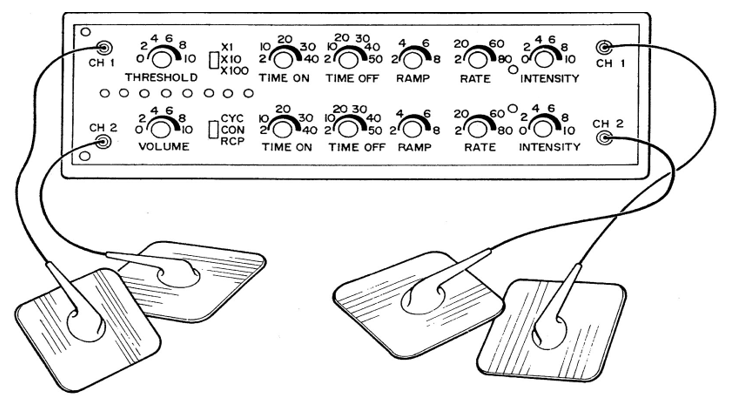
\includegraphics[width=0.7\linewidth]{figs/Fig_c3/ian_f3}
    \caption{Interface analógica e eletrodos do estimulador proposto na patente  \cite{Reiss1996CombinationSystem}.}
    \label{fig:ian_f3}
\end{figure*}

\vspace{0.3cm}
% fig 4
\begin{figure*}[h]
    \centering %
    \small %
    \def\svgwidth{0.9\columnwidth}% Código LATEX define o tamanho da figura 
    \import{figs/Fig_c3/}{gem_f4.pdf_tex}
    \caption{Gerador de sinal (a) e etapa de potência com transformador (b). Estimulador em  \cite{Phillips1980ApparatusTES}.}
    \label{fig:gem_f4}
\end{figure*}

No ano de 1989 foi introduzida a eletroestimulação funcional no Brasil pelo Professor Sergio Lianza da Santa e, com a ajuda técnica dos Doutores Franco Gracanin e Tajed Badj da Universidade de Lubljana (ex-Iugoslávia), foi desenvolvido o primeiro estimulador elétrico de fabricação nacional \cite{Santos1995EquipamentosFuncional}. Alguns anos depois, a técnica de estimulação elétrica para restauração do movimento foi usada por primeira vez em 1991 no Hospital de Clinicas de Porto Alegre visando sua aplicação em marcha assistida \cite{Santos1995EquipamentosFuncional}.

\section{SISTEMAS CONTEMPORÂNEOS DE ELETROESTIMULAÇÃO}

No contexto mundial, em meados dos anos 90 a evolução das tecnologias em eletrônica permitiu o desenvolvimento de novos dispositivos de estimulação \cite{Wu2002AApplications}. Assim, os eletroestimuladores evoluíram em cada um dos seus módulos, por exemplo interfaces de usuário digitais, circuitos de menor tamanho, até aparelhos portáteis. Como resultado disto, um grande número de dispositivos tem sido desenvolvido para pesquisa, aplicações clinicas e esportivas \cite{Popovic2004CompexApplications}.

Muitos desses dispositivos foram desenvolvidos para tarefas específicas (para um só tipo de tratamento ou restauração de uma só função corporal \cite{Brunetti2011EnhancingProject,Souza2017PowerSystems}).  %Brunetti 2011;Souza 2017;
Desta forma, se um usuário desejasse utilizar o dispositivo para tarefas diferentes daquelas que foi projetado, iria precisar modificar o hardware, o software ou ambos. Realizar isto ficava impraticável em dispositivos comerciais, portanto muitos pesquisadores se viram forçados a direcionar suas energias ao desenvolvimento de equipamentos de estimulação customizados, visando o seu uso em várias tarefas. Em consequência, muitos dispositivos de estimulação foram feitos e como tal, diversas soluções foram empregadas para seu desenvolvimento \cite{Ilic1994ASystems, Popovic2001CompexApplications}. %Ilic 1994;Popovic 2001;

Como apresentado no capítulo anterior, um sistema de eletroestimulação típico geralmente possui os módulos mostrados na Figura \ref{fig:se_f9}. Desta forma, a seguir se apresenta uma revisão destes módulos.

\subsection{Interface de controle}
Interface de controle é o meio pelo qual o usuário final do dispositivo de estimulação controla as funcionalidades do mesmo. Nesse contexto, neste documento a interface de controle identifica-se como o conjunto de interface de usuário e de controle. 

Independentemente do tipo de aplicação (pé caído, controle de agarre, neuropróteses, etc.) em que um estimulador seja usado, sempre é necessário controlar não só os parâmetros de estimulação, mas possivelmente também outros aspectos como o tipo de terapia, o tempo de sessão e finalmente a quantidade de canais de estimulação ativados \cite{Gaiotto2012EstimuladorEletricamente}. Os parâmetros recebidos como informações de entrada pela interface de controle normalmente são administrados pela unidade de controle que gerencia o sistema de eletroestimulação.

A interface de controle pode estar implementada como uma interface externa ao eletroestimulador, podendo ser um microcomputador, teclado matricial, elementos analógicos de ajustes (potenciômetros), telas sensitivas, botões ou até mesmo dispositivos sem fio \cite{Gaiotto2012EstimuladorEletricamente}. Nesse contexto, a utilização de estratégias digitais (e.g. microcomputador, dispositivos sem fio, entre outros), determinam o ponto de partida à incorporação de interfaces digitais nos eletroestimuladores \cite{Bijak2002TheParaplegia}.

Nesse contexto, no início dos anos 90 começaram a ser desenvolvidos os primeiros estimuladores controlados por meio de Interfaces de Controle Digitais (\acrshort{ICD}) \cite{Kaczmarek1991ASystem}. Este tipo de interface tem uma grande vantagem com relação a Interfaces de Controle Analógicas (\acrshort{ICA}), pois está em geral ocupa maior espaço físico no dispositivo. Por exemplo, a \acrshort{ICD} pode conter no mesmo espaço diversos tipos de controles ou até não existir fisicamente, ou seja, o dispositivo é controlado por um outro dispositivo externo, como por exemplo por meio de um software em microcomputador \cite{Wu2002AApplications, Bijak2002TheParaplegia}. 

Além das classificações em \acrshort{ICD} e \acrshort{ICA}, as interfaces de controle podem também ser classificadas como mistas, i.e. contendo elementos digitais e analógicos de interface. Do mesmo modo, as \acrshort{ICD} podem ser classificadas em três tipos: \acrshort{ICD} embarcada no dispositivo, \acrshort{ICD} externa (e.g. baseada em microcomputador, dispositivo móvel) ou mista.

Em relação ao tema, vale comentar o dispositivo produzido por Popovic et al. no final dos anos 90. Este estimulador foi concebido como um novo estimulador elétrico transcutâneo portátil e programável com uma ampla gama de aplicações de estimulação elétrica. A sua grande vantagem era que podia ser utilizado para diversas aplicações como neuropróteses, dispositivos de avaliação neurológica, sistemas de exercício e estudos fisiológicos. A sua desvantagem era causada pelo sistema de controle e a sua \acrshort{ICD} de natureza complexa (possuía uma \acrshort{ICD} mista) e, portanto, o usuário final deveria ter um conhecimento relativamente amplo para usá-lo. Este eletroestimulador foi usado para pesquisa e em alguns ensaios clínicos \cite{Popovic2001CompexApplications, Popovic2005ModularSystem}.

Bijak et al. também implementaram uma \acrshort{ICD} mista (ver Figura \ref{fig:see_f5} e Figura \ref{fig:icd_f6}) que fazia parte de um sistema de restauração das funções de caminhada na paraplegia espástica \cite{Bijak2002TheParaplegia}. Este sistema usa uma \acrshort{ICD} baseada em um computador palmtop e um PC para controlar o eletroestimulador. No palmtop é possível carregar as configurações de sequências de estimulação para ficar em pé, caminhar ou se sentar. Esta interface foi usada pela facilidade que oferecia para acessar a uma base de dados e selecionar na tela sensível ao toque diferentes funcionalidades, assim como manipular vários parâmetros de estimulação. Na Figura \ref{fig:icd_f6} pode-se observar a \acrshort{ICD} desenvolvida.

\vspace{0.3cm}
%fig 5
\begin{figure*}[h]
    \centering %
    \small %
    \def\svgwidth{0.6
    \columnwidth}% Código LATEX define o tamanho da figura 
    \import{figs/Fig_c3/}{see_f5.pdf_tex}
    \caption{Sistema de eletroestimulação que usa ICD misto (adaptada de  \cite{Bijak2002TheParaplegia}).}
    \label{fig:see_f5}
\end{figure*}

Outro tipo de \acrshort{ICD} junto com \acrshort{ICA} muito usada em sistemas de eletroestimulação é a Interface Homem Máquina (\acrshort{IHM}) que se baseia em um display de cristal líquido (\acrshort{LCD}) que junto a um teclado gerenciam o funcionamento do dispositivo. Autores como Alonso et al. \cite{Alonso2007DesignEffects} e Teixeira et al. \cite{Teixeira1998SistemaMicrocontrolado} usam este tipo de interface de controle. Velloso et al. \cite{Velloso2007AFES} implementou uma \acrshort{ICD} baseada em um dispositivo portátil com interface USB que possui portas de entrada/saída digitais programáveis conectado a um computador junto à ferramenta LabVIEW. 

É de esclarecer que em alguns estimuladores a interface de controle mista a componentes discretos podem ter a função de controlar diretamente o dispositivo sinal gerado, como no caso de Cheng et al., onde o controle da frequência é feito ajustando o valor de resistência de um potenciômetro analógico \cite{Cheng2004DevelopmentStimulation}. Isto reduz a demanda de processamento em microprocessadores ou microcontroladores \cite{Gaiotto2012EstimuladorEletricamente}. Em muitos outros sistemas, porém, usa-se uma interface de controle dependente de uma unidade de controle, onde esta última é responsável pelo gerenciamento e processamento de todos os componentes do sistema de eletroestimulação \cite{ Wu2002AApplications, Popovic2004CompexApplications, Souza2017PowerSystems,Bijak2002TheParaplegia, Martins2008DeselvolvimentoArbitraria}. 

% Fig 6
\begin{figure*}
    \centering %
    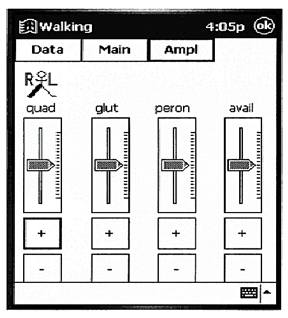
\includegraphics[width=0.35\linewidth]{figs/Fig_c3/icd_f6}
    \caption{Interface gráfica de usuário ou \acrshort{ICD} em dispositivo móvel (palmtop)  \cite{Bijak2002TheParaplegia}.}
    \label{fig:icd_f6}
\end{figure*}

\subsection{Unidade de controle}

A unidade de controle (\acrshort{UC}) é responsável pelo processamento de dados e gerenciamento de todos recursos de software e hardware de um sistema de eletroestimulação. A \acrshort{UC} recebe como entrada informações de diferentes componentes, como botões, teclados, sensores de diversos tipos (e.g. acelerômetros, goniômetros), potenciômetros. Pode também possuir conectividade por meio de diversas padrões e protocolos, \acrshort{USB}, \acrshort{I2C}, \acrshort{UART}, \acrshort{SPI}, Bluetooth, entre outros, com outros módulos e componentes externos. Tais conexões permitem que a \acrshort{UC} envie e receba informação de dentro e de fora do dispositivo. 

Tipicamente o usuário usa uma interface de controle para interagir com a \acrshort{UC}, permitindo manipular diferentes caraterísticas do sistema \cite{Souza2012EstagioFuncional, Wu2002AApplications, Popovic2004CompexApplications, Masdar2012DevelopmentInjuries}. Em sistemas atuais, geralmente a \acrshort{UC} é implementada em microcontroladores ou plataformas de desenvolvimento, como no caso de Johnsen et al. \cite{Johnsen2011DesignPost-fracture} que usou a plataforma de desenvolvimento baseada em Arduino para seu eletroestimulador, no qual visava diminuir a atrofia muscular do antebraço post-fratura, ou O’Keefffe et al. \cite{OKeeffe2002AApplications} que usa um microcontrolador como \acrshort{UC} e gerador de sinal no seu estimulador versátil para aplicações de pesquisa em pé caído. Nesse último caso foram implementados algoritmos de controle que usam as informações de sensor de marcha para se adaptar à velocidade da caminhada do paciente, adaptando os parâmetros de estimulação segundo seja necessário.

Outro exemplo de \acrshort{UC} é apresentado em um sistema de neuroestimulação elétrica com forma de onda arbitrária desenvolvido por pesquisadores da Universidade Federal de Minas Gerais (\acrshort{UFMG}) \cite{Martins2008DeselvolvimentoArbitraria}. Eles usaram para implementar a \acrshort{UC} uma plataforma de desenvolvimento baseada em um processador digital de sinais (em inglês Digital Signal Processor, \acrshort{DSP}). Sua \acrshort{UC} tem várias funções como gerar um sinal analógico que posteriormente controla uma fonte de corrente, administrar a comunicação entre o sistema de estimulação e uma interface gráfica em um computador e aferir, por meio de uma chave do tipo push-button, a informação do voluntário à percepção do estímulo \cite{Martins2008DeselvolvimentoArbitraria}. Na Figura \ref{fig:seu_f7} se apresenta o dispositivo desenvolvido e nela é indicada a \acrshort{UC}.

%fig 7
\begin{figure*}
    \centering %
    \small %
    \def\svgwidth{0.4
    \columnwidth}% Código LATEX define o tamanho da figura 
    \import{figs/Fig_c3/}{seu_f7.pdf_tex}
    \caption{Unidade de controle do estimulador da \acrshort{UFMG}   \cite{Martins2008DeselvolvimentoArbitraria}.}
    \label{fig:seu_f7}
\end{figure*}

\subsection{Gerador de sinais}
Este componente está presente em todos os dispositivos de estimulação elétrica e é responsável pela produção de sequências de pulsos elétricos de baixa amplitude (sinais de baixa tensão ou corrente). Tipicamente, o gerador de sinais pode ser composto por componentes das seguintes naturezas: circuito oscilador, microcontrolador com \acrshort{PWM}, conversor digital-analógico, entre outros.  É no gerador de sinais em que alguns parâmetros de baixo nível do sinal de saída são controlados, notadamente a amplitude, largura de pulso e frequência \cite{Cheng2004DevelopmentStimulation, Wu2002AApplications}.

Wu et al. \cite{Wu2002AApplications}, por exemplo, usaram um \acrshort{DSP} como gerador de sinais com formatos de onda arbitrários. Ele também usa o \acrshort{DSP} como \acrshort{UC}. Já alguns outros dispositivos possuem um circuito modulador que gera um sinal modulado usando dois sinais: um sinal de alta frequência produzido pelo gerador de sinal e outro que comanda a geometria da envoltória. A interação entre estes dois componentes (o gerador de sinal e o modulador) permite criar sinais de estimulação com formas de onda diversas \cite{Wu2002AApplications, Nogueira2017TheStimulator,KhosravaniSanaz2011DevelopingSystem}. Um exemplo de sinal modulado se mostra na Figura \ref{fig:ges_f8}.

Note-se que não existe um padrão para a implementação do gerador de sinal/modulador, pois seu desenvolvimento varia de acordo com o tipo de aplicação, disponibilidade de componentes ou até pode ser uma escolha subjetiva do projetista do equipamento \cite{Souza2017PowerSystems, Popovic2004CompexApplications}.

\vspace{0.3cm}
%fig 8
\begin{figure*}
    \centering %
    \small %
    \def\svgwidth{0.42
    \columnwidth}% Código LATEX define o tamanho da figura 
    \import{figs/Fig_c3/}{ges_f8.pdf_tex}
    \caption{Geração de sinal modulada usando modulação por amplitude de pulso, (a) sinal de modulação, (b) Sinal da portadora, (c) Sinal modulada   \cite{Martins2008DeselvolvimentoArbitraria}.}
    \label{fig:ges_f8}
\end{figure*}

% Sub section %%%%%%%%%%%%%%%%%%%%%%%%%%%%%%%%%%%%%
\subsection{Estágio de potência de saída}
\label{sub_cap:eps}

O estágio de potência de saída (\acrshort{EPS}) é o responsável por amplificar o sinal de eletroestimulação proveniente do gerador de sinal a um sinal de alto nível de tensão ou corrente, chamado também de estímulo elétrico. O estímulo elétrico finalmente é aplicado por meio de eletrodos de superfície em uma carga que é identificada como o conjunto pele-músculo-nervo do paciente \cite{Souza2017PowerSystems}.

Como descrito no Cap. \ref{sec:cap2}, o estímulo elétrico pode ser aplicado no tecido neuromuscular de duas formas: por tensão constante ou por corrente constante. Escolher a forma de aplicá-lo determina o desenho do circuito do \acrshort{EPS}. Outra caraterística importante que determina a topologia do circuito do \acrshort{EPS} é se este irá trabalhar com sinais monofásicos ou bifásicos \cite{Ilic1994ASystems}. 

Além disso, um sistema de eletroestimulação pode comportar um ou vários canais de estimulação, os quais dependem de um ou mais \acrshort{EPS}. Desta forma, o \acrshort{EPS} no módulo de estimulação é o componente mais relevante em um sistema típico de eletroestimulação \cite{Ilic1994ASystems, Velloso2007SistemaFES-PEB}. Quando um estimulador tem vários canais, por exemplo, estes podem possuir diferentes níveis de interdependência. Na situação na qual os canais possuem maior nível de dependência, todos os canais possuem os mesmos parâmetros de estimulação, com a diferença de que eles são ativados de forma sequencial chaveando um único \acrshort{EPS}. Já nos casos em que os canais possuem completa independência, cada canal pode possuir configurações diferentes dos parâmetros de estimulação, assim como independência na temporização do sinal \cite{Faria2006ImplementacaoMedulares,Wu2002AApplications, Quark2013DualpexNeuromuscular}. 

A seguir são apresentados os trabalhos que usam diferentes tipos de \acrshort{EPS}. A Tabela \ref{tab:eps1} mostra um resumo das caraterísticas mais relevantes dos circuitos de \acrshort{EPS} contemporâneos. Basicamente os circuitos do \acrshort{EPS} foram agrupados em quatro categorias de acordo com o componente principal de saída da topologia: baseada em transformador para elevação de tensão, baseada em ponte H, baseada em amplificadores operacionais e conversores tensão-corrente e, finalmente, baseada em espelho de corrente. Na Tabela \ref{tab:eps1} o item parâmetros de estimulação apresenta somente os parâmetros fornecidos pelos autores. Além disso, em todas as topologias são usadas a seguinte nomenclatura: saída do gerador e \acrshort{$R_{CARGA}$}, para simbolizar, respectivamente, a entrada do sinal de controle do \acrshort{EPS} e a resistência do conjunto eletrodo-pele-tecido neuromuscular.

\newpage
% Please add the following required packages to your document preamble:
% \usepackage[table,xcdraw]{xcolor}
% If you use beamer only pass "xcolor=table" option, i.e. \documentclass[xcolor=table]{beamer}
\begin{table}[H]
    \centering
    \caption{Resumo dos circuitos do \acrshort{EPS} dos artigos analisados. Os artigos de cada grupo foram ordenados por ano, do mais antigo ao mais recente.}
    \begin{tabular}{cccl}
    \hline
    \rowcolor[HTML]{DBDBDB} 
    \textbf{Referência}        & \textbf{\begin{tabular}[c]{@{}c@{}}Saída controlada \\ por V  ou I\end{tabular}} & \textbf{\begin{tabular}[c]{@{}c@{}}Tipo da topologia da saída\\ M ou B\end{tabular}}                             & \multicolumn{1}{c}{\cellcolor[HTML]{DBDBDB}\textbf{\begin{tabular}[c]{@{}c@{}}Parâmetros de \\ estimulação (máx)\end{tabular}}} \\ \hline
    Cheng et al. \cite{Cheng2004DevelopmentStimulation}      & I                                                                                & B (baseado em T)                                                                                                 & \begin{tabular}[c]{@{}l@{}}f= 200 Hz\\ I= 100 mA\\ V= 200V\end{tabular}                                                         \\ \hline
    Souza et al. \cite{Souza2012EstagioFuncional}      & I                                                                                & B (baseado em T)                                                                                                 & \begin{tabular}[c]{@{}l@{}}PW= 250 $\mathrm{\mu}$s\\ f= 200 Hz\\ I= 100 mA\end{tabular}                                                      \\ \hline
    Chen et al. \cite{Chen2013ADataset}       & V                                                                                & M (baseado em T)                                                                                                 & \begin{tabular}[c]{@{}l@{}}PW= 400 $\mathrm{\mu}$s\\ f= 40 Hz\\ V= 150V\end{tabular}                                                         \\ \hline
    Hongen et al. \cite{Hongen2011DevelopmentRehabilitation}     & I                                                                                & M/B (baseado em Ponte H)                                                                                         & \begin{tabular}[c]{@{}l@{}}PW= 65535 $\mathrm{\mu}$s \\ f= 1000 Hz\\ I= 300 mA\\ V= 600 V\end{tabular}                                       \\ \hline
    Gaiotto et al. \cite{Gaiotto2012EstimuladorEletricamente}    & V                                                                                & M/B (baseado em Ponte H)                                                                                         & \begin{tabular}[c]{@{}l@{}}PW= 65535 $\mathrm{\mu}$s \\ f= 1000 Hz\\ I= 300 mA\\ V= 600 V\end{tabular}                                       \\ \hline
    Masdar et al. \cite{Masdar2012DevelopmentInjuries}     & I                                                                                & \begin{tabular}[c]{@{}c@{}}M/B (baseado em amp op. como\\  CTC)\end{tabular}                                     & \begin{tabular}[c]{@{}l@{}}PW= 500 $\mathrm{\mu}$s \\ I= 120 mA\end{tabular}                                                                 \\ \hline
    Willand et al. \cite{Willand2008DesignFES.}    & I                                                                                & \begin{tabular}[c]{@{}c@{}}M (baseado em amp op. e \\ CTC com transistor)\end{tabular}                           & \begin{tabular}[c]{@{}l@{}}PW= 10 ms \\ f= 15 kHz\\ I= 125 mA\\ V= 300 V\end{tabular}                                           \\ \hline
    Brunetti et al. {[}65{]}   & I                                                                                & \begin{tabular}[c]{@{}c@{}}B (baseado em amp op. de \\ transcondutância e chaveamento \\ de canais)\end{tabular} & \begin{tabular}[c]{@{}l@{}}PW= 5 ms \\ f= 100 Hz\\ I= 125 mA\\ V= 250 V\end{tabular}                                            \\ \hline
    Lima et al. \cite{DeLima2002AControl}       & I                                                                                & M (baseado em EC)                                                                                                & \begin{tabular}[c]{@{}l@{}}PW= 1 ms\\ f= 10 Hz\\ I= 20 mA\\ V= 220 V\end{tabular}                                               \\ \hline
    Wu et al. \cite{Wu2002AApplications}         & I                                                                                & M/B (baseado em EC)                                                                                              & \begin{tabular}[c]{@{}l@{}}PW= 50 $\mathrm{\mu}$s \\ f=100 Hz\\ I= 110 mA\\ V= 300 V\end{tabular}                                            \\ \hline
    Khosravani et al. \cite{KhosravaniSanaz2011DevelopingSystem} & I                                                                                & M/B (baseado em EC)                                                                                              & \begin{tabular}[c]{@{}l@{}}f= 50 Hz\\ I= 150 mA\end{tabular}                                                                    \\ \hline
    \multicolumn{4}{l}{\begin{tabular}[c]{@{}l@{}}T - Transformador, CTC - Conversor Tensão-Corrente, EC – Espelho de corrente, PW – largura de \\ pulso, f – frequência, I – Intensidade, V – Voltagem, M - Monofásica, B - Bifásica\end{tabular}} 
    \\ \hline
    \end{tabular}
    \label{tab:eps1}
\end{table}

\subsection*{Topologia dos \acrshort{EPS} baseadas em transformador}

Algumas topologias dos EPS baseadas em transformador para elevação de tensão são ilustradas nas Figura \ref{fig:chg_f9}, Figura \ref{fig:sza_f10} e Figura \ref{fig:chn_f11}. Nos circuitos ilustrados na Figura \ref{fig:chg_f9} a Figura \ref{fig:chn_f11}, além do transformador, é utilizado um transistor que chaveia a ativação do enrolamento primário do transformador, resultando em pulsos de alta tensão no enrolamento secundário. No caso de Cheng et al. e Souza et al., a topologia do \acrshort{EPS} foi desenhada para realizar a estimulação por corrente. Já, no caso de Chen et al., a topologia do \acrshort{EPS} foi desenhada para realizar a estimulação por tensão. 


%Figura 3.9 – Circuito baseados em transformador com saída de corrente (adaptado de [76]).
\begin{figure*}[h]
    \centering %
    \small %
    \def\svgwidth{0.75
    \columnwidth}% Código LATEX define o tamanho da figura 
    \import{figs/Fig_c3/}{chg_f9.pdf_tex}
    \caption{Circuito baseados em transformador com saída de corrente (adaptado de \cite{Cheng2004DevelopmentStimulation}).}
    \label{fig:chg_f9}
\end{figure*}

%Figura 3.10 – Circuito baseados em transformador com saída de corrente (adaptado de [84]).
\begin{figure*}[h]
    \centering %
    \small %
    \def\svgwidth{0.78
    \columnwidth}% Código LATEX define o tamanho da figura 
    \import{figs/Fig_c3/}{sza_f10.pdf_tex}
    \caption{Circuito baseados em transformador com saída de corrente (adaptado de \cite{Souza2012EstagioFuncional}).}
    \label{fig:sza_f10}
\end{figure*}

%Figura 3.11 – Circuito baseado em transformador com saída de tensão (adaptado de [85]).
\begin{figure*}
    \centering %
    \small %
    \def\svgwidth{0.6
    \columnwidth}% Código LATEX define o tamanho da figura 
    \import{figs/Fig_c3/}{chn_f11.pdf_tex}
    \caption{Circuito baseados em transformador com saída de tensão (adaptado de \cite{Chen2013ADataset}).}
    \label{fig:chn_f11}
\end{figure*}

No circuito proposto por Chang et al., ilustrado na Figura \ref{fig:chg_f9}, existem quatro etapas identificadas pelos amplificadores operacionais OP1A, OP1B, OP2A e OP2B. O OP1A é usado como amplificador de erro, o OP1B é um amplificador de sinal para controlar o transformador $T_{1}$, o OP2A e OP2B fecham o laço do circuito realimentando o amplificador de erro de acordo com a corrente na saída de $T_{1}$, o que permite conferir a corrente de saída que será passada na carga (RCARGA). Finalmente, a amplitude do pulso de corrente é controlada pelo potenciômetro $R_{V2}$. Para Cheng et al., o transformador ($T_{1}$) é o componente de maior tamanho e o mais custoso do estágio de potência. O mesmo acontece com o circuito do Souza et al. Isto compromete a portabilidade e a inclusão de mais canais de estimulação.

O circuito proposto por Souza et al. é uma versão melhorada do circuito proposto por Cheng et al. onde a principal melhora é fornecer um isolamento completo entre o paciente e o circuito. Quatro transistores ($T_{1}$, $T_{2}$, $T_{3}$ e $T_{4}$) foram colocados em configuração darlington com a finalidade de reforçar o fornecimento de corrente (bidirecional) que energiza o enrolamento primário do transformador $T_{R1}$, resultando em um melhor fornecimento de corrente no secundário. É usado também um transformador amostrador $T_{R2}$ na realimentação para realizar a comparação do sinal de saída com o sinal do gerador depois de passar por uma amplificação no OP2A. Uma caraterística importante deste circuito é a conexão do resistor $R_{7}$ em paralelo com a $R_{CARGA}$. Ele atua como proteção para o \acrshort{EPS} no caso de desconexão acidental ou intencional dos eletrodos do paciente, ou seja, desconexão da $R_{CARGA}$.

O circuito implementado por Chen et al. é mais simples quando comparado com o proposto por Cheng et al. e Souza et al. Na saída do enrolamento secundário do transformador a tensão pode chegar aos 800V, portanto ela é limitada a 150V com o diodo $D_{1}$ na Figura \ref{fig:chn_f11}. Contudo, Cheng et al. não evidenciam em que valor de carga e a máxima corrente com que o circuito trabalha.

% segundo grupo
\subsection*{Topologia dos \acrshort{EPS} baseadas em ponte H}

Na segunda categoria da Tabela \ref{tab:eps1} destacam-se os \acrshort{EPS} que usam ponte H para criar um estímulo elétrico bifásico a partir de uma ou duas fontes de tensão/corrente.
No caso de Hongen et al., a ponte H é controlada por quatro chaves (S1-S4), como mostrado na Figura \ref{fig:hgn_f12} (a) e o sinal do estímulo elétrico vem de duas fontes de corrente controladas por tensão \cite{Hongen2011DevelopmentRehabilitation}. O EPS proposto por Hongen et al. chaveia entre duas fontes de corrente (I1 e I2) segundo a lógica mostrada na Figura \ref{fig:hgn_f12} (b) e desta forma é criado o sinal do estímulo elétrico da Figura \ref{fig:hgn_f12} (c).

%Figura 3.12 – Circuito do EPS utilizando ponte H (a), relação de chaveamento entre S1-S4 e I1-I2 (b), e sinal do estímulo elétrico na carga (c) (adaptado de [86]).

\begin{figure*}
    \centering %
    \small %
    \def\svgwidth{0.9
    \columnwidth}% Código LATEX define o tamanho da figura 
    \import{figs/Fig_c3/}{hgn_f12.pdf_tex}
    \caption{Circuito do EPS utilizando ponte H (a), relação de chaveamento entre S1-S4 e I1-I2 (b), e sinal do estímulo elétrico na carga (c) (adaptado de \cite{Hongen2011DevelopmentRehabilitation}).}
    \label{fig:hgn_f12}
\end{figure*}

Gaiotto et al. desenvolveu um estimulador elétrico neuromuscular bifásico com saída em ponte H controlado por tensão \cite{Gaiotto2012EstimuladorEletricamente}. A Figura \ref{fig:gto_f13} apresenta a composição básica da ponte H implementada no \acrshort{EPS}.

%Figura 3.13 – Diagrama de blocos do EPS com ponte H (adaptado de [69]).
\begin{figure*}
    \centering %
    \small %
    \def\svgwidth{0.9
    \columnwidth}% Código LATEX define o tamanho da figura 
    \import{figs/Fig_c3/}{gto_f13.pdf_tex}
    \caption{Diagrama de blocos do EPS com ponte H (adaptado de \cite{Gaiotto2012EstimuladorEletricamente}).}
    \label{fig:gto_f13}
\end{figure*}

Gaiotto et al. usou transistores MOSFET na implementação da ponte H, permitindo que EPS possa funcionar com altas tensões e altas valores de corrente que, em suma, vão depender da fonte de alta tensão que vai polarizar a ponte H. A topologia do \acrshort{EPS} proposto por Gaiotto et al. comporta um canal de estimulação. Os MOSFET $T_{1}$ e $T_{2}$ junto com o driver de meia ponte 1 criam o lado positivo do sinal de estimulação e o $T_{3}$, $T_{4}$ e o driver de meia ponte 2 o lado negativo. O sinal do gerador permite chavear a fonte $V_{CC}$ em direção à $R_{CARGA}$, ativando os drivers de meia ponte de forma alternada, criando um sinal bifásico ou monofásico. Os drivers de meia ponte foram usados para fornecer o \textit{dead} time entre o acionamento dos transistores da meia ponte, garantindo que as capacitâncias dos terminais do \textit{gate} dos MOSFETS sejam descarregadas, prevenindo assim a ocorrência de um curto-circuito momentâneo quando está se realizando a alternância de ativação pelo sinal de controle \cite{Gaiotto2012EstimuladorEletricamente}.

% 3er grupo
\subsection*{Topologia dos \acrshort{EPS} baseadas em amplificadores operacionais}
Na terceira categoria da Tabela \ref{tab:eps1} destacam-se os \acrshort{EPS} implementados usando amplificadores operacionais conectados diretamente na carga. 

Masdar et al. \cite{Masdar2013CurrentStimulation} usou duas fontes de alta tensão ($V_{1}$ e $V_{2}$ na Figura \ref{fig:msd_f14}) para energizar o \acrshort{EPS} formado por um conversor de tensão-corrente baseado em um amplificador operacional que opera com tensões de até 60V (OP2) e consegue fornecer até 3A na sua saída. Dispondo de duas fontes conectadas em série, Masdar implementou formas de onda monofásicas e bifásicas. Finalmente, o sinal do gerador usado por Masdar é gerado em um \acrshort{DAC} com saída monofásica e é convertida em bifásico por meio do amplificador operacional OP1B para logo entrar como sinal controle no OP2 que produz o estimulo elétrico que é entregue à $R_{CARGA}$.

Willand et al. \cite{Willand2008DesignFES.} utiliza um conversor de tensão-corrente baseado em um transistor de alta tensão $T_{1}$, um amplificador operacional e uma resistência de referencia (R1 na Figura 3.15). O sinal do gerador é convertido em corrente por meio do $R_{1}$ produzindo só sinais monofásicos. A corrente que passa por $R_{1}$ ira circular igualmente por $R_{CARGA}$. O transistor $T_{2}$ é usado para ativar e desativar o estimulo elétrico que é fornecido à $R_{CARGA}$ por meio de um controle de ativação e, finalmente, um opto-acoplador é usado para isolar $R_{CARGA}$ do resto do circuito do estimulador.

\vspace{0.3cm}

% Figura 3.14 – Circuito do EPS usando o conversor de tensão-corrente (adaptado de [78]).
\begin{figure*}[h]
    \centering %
    \small %
    \def\svgwidth{0.9
    \columnwidth}% Código LATEX define o tamanho da figura 
    \import{figs/Fig_c3/}{msd_f14.pdf_tex}
    \caption{Circuito do EPS usando o conversor de tensão-corrente (adaptado de \cite{Masdar2012DevelopmentInjuries}).}
    \label{fig:msd_f14}
\end{figure*}

% Figura 3.15 – Circuito do EPS usando o conversor de tensão-corrente (adaptado de [87]).
\begin{figure*}
    \centering %
    \small %
    \def\svgwidth{0.45
    \columnwidth}% Código LATEX define o tamanho da figura 
    \import{figs/Fig_c3/}{wad_f15.pdf_tex}
    \caption{Circuito do EPS usando o conversor de tensão-corrente (adaptado de \cite{Willand2008DesignFES.}).}
    \label{fig:wad_f15}
\end{figure*}

Outra topologia de \acrshort{EPS} em que se usa amplificador operacional é a proposta por Brunetti et al. \cite{Brunetti2011EnhancingProject}. A diferença principal com os dois \acrshort{EPS} anteriores baseados em amplificador operacional é que Brunetti et al. usam um amplificador operacional de transcondutância (\acrshort{AOT}) de alta tensão (U8A na Figura \ref{fig:bni_f16}). Do mesmo modo que Masdar, o \acrshort{AOP} é usado como conversor tensão-corrente sendo conectado diretamente na carga, compondo o \acrshort{EPS}. Para energizar o \acrshort{EPS} foi usado um conversor CC/CC que eleva a tensão até 250V. A Figura \ref{fig:bni_f16} mostra o circuito do \acrshort{EPS} proposto por Brunetti et al. \cite{Brunetti2011EnhancingProject}.

%Figura 3.16 – Circuito do EPS usando o conversor de tensão-corrente com amplificador operacional de transcondutância de alta tensão (adaptado de [65]).
\begin{figure*}[h]
    \centering %
    \small %
    \def\svgwidth{0.57
    \columnwidth}% Código LATEX define o tamanho da figura 
    \import{figs/Fig_c3/}{bni_f16.pdf_tex}
    \caption{Circuito do EPS usando o conversor de tensão-corrente com amplificador operacional de transcondutância de alta tensão (adaptado de \cite{Brunetti2011EnhancingProject}).}
    \label{fig:bni_f16}
\end{figure*}

% 4to grupo
\subsection*{Topologia dos \acrshort{EPS} baseadas em espelhos de corrente}
Na última categoria da Tabela \ref{tab:eps1} estão os EPS implementados usando espelhos de corrente. O espelho de corrente é uma topologia muito usada em diversos dispositivos eletrônicos. Em sistemas de eletroestimulação o espelho de corrente é usado no EPS para espelhar uma corrente de referência na $R_{CARGA}$ mantendo-a constante, assim como melhorar o seu controle em diferentes tipos de formato de onda \cite{Kaczmarek1991ASystem, Souza2017PowerSystems, Boylestad2013DispositivosCircuitos}. %[66, 71, 89]. Kaczmarek 1991;Souza 2017;Boylestad 2013;

A quantidade de corrente que pode ser aplicada na carga depende diretamente da fonte com que é energizado o espelho, pois supondo que é o circuito usa componentes ideais, por lei de Ohm se a corrente é constante e a resistência muda, a tensão obrigatoriamente tem que acompanhar essa mudança modificando seu valor para manter a dita corrente constante. Em essência esse é o trabalho do espelho de corrente \cite{Boylestad2013DispositivosCircuitos}. %[89].

Nas Figura \ref{fig:lma_f17} a Figura \ref{fig:khi_f19} estão identificados nas caixas azuis os EPS baseados em espelho de corrente dos autores Lima et al. \cite{DeLima2002AControl}, Wu et al. \cite{Wu2002AApplications} e Khosravani et al. \cite{KhosravaniSanaz2011DevelopingSystem}, respectivamente.

%Figura 3.17 – Circuito baseados em espelho de corrente com controle de ativação (adaptado de [88]).
\begin{figure*}[h]
    \centering %
    \small %
    \def\svgwidth{0.6
    \columnwidth}% Código LATEX define o tamanho da figura 
    \import{figs/Fig_c3/}{lma_f17.pdf_tex}
    \caption{Circuito baseados em espelho de corrente com controle de ativação (adaptado de \cite{DeLima2002AControl}).}
    \label{fig:lma_f17}
\end{figure*}

O EPS implementado por Lima et al. \cite{DeLima2002AControl} usa um espelho de corrente cascode auto-polarizado composto de transistores MOSFET como mostrado na Figura \ref{fig:lma_f17}. A tensão total que polariza o \acrshort{EPS} é o resultado das tensões: $V_{t}= V_{gs} - V_{GS3} - V_{GS1}$, onde $V_{gs}$ é o sinal do gerador, $V_{GS_{X}}$ representa as quedas de tensão entre a porta e a fonte dos MOSFETs $T_{1}$ e $T_{3}$.  A corrente $I_{ref}$ que forma o estímulo elétrico é o resultado da tensão $I_{ref}  = \frac{V_{t}}{R_{5}}$. Finalmente, com o controle de ativação são criados os pulsos do estimulo elétrico quando o $T_{5}$ é ativado/desativado.

% Figura 3.18 – Circuitos baseados em espelho de corrente (adaptado de [81]).
\begin{figure*}
    \centering %
    \small %
    \def\svgwidth{0.7
    \columnwidth}% Código LATEX define o tamanho da figura 
    \import{figs/Fig_c3/}{wuc_f18.pdf_tex}
    \caption{Circuitos baseados em espelho de corrente (adaptado de \cite{Wu2002AApplications}).}
    \label{fig:wuc_f18}
\end{figure*}

% Figura 3.19 – Circuito baseados em espelho de corrente de Wilson (caixa azul) junto com um circuito de comutação de Howland (caixa laranja) (adaptado de [81]).
\begin{figure*}
    \centering %
    \small %
    \def\svgwidth{1
    \columnwidth}% Código LATEX define o tamanho da figura 
    \import{figs/Fig_c3/}{khi_f19.pdf_tex}
    \caption{Circuito baseados em espelho de corrente de Wilson (caixa azul) junto com um circuito de comutação de Howland (caixa laranja) (adaptado de \cite{KhosravaniSanaz2011DevelopingSystem}).}
    \label{fig:khi_f19}
\end{figure*}

Outro \acrshort{EPS} que também usa uma topologia de espelho de corrente é o proposto por Wu et al. \cite{Wu2002AApplications}. Em suma este \acrshort{EPS} é baseado em duas etapas: o conversor tensão-corrente e o espelho de corrente de Wilson (\acrshort{ECW}). O conversor é implementado usando a Arquitetura de Howland que cria uma corrente de referencia ($I_{ref}$) a partir do sinal do gerador, como mostrado na Figura \ref{fig:wuc_f18}, por meio dos amplificadores operacionais OP1A e OP2B para o sinal positivo e negativo, respectivamente. O sinal do gerador é, então, o sinal de controle do \acrshort{EPS}. 

O espelho de corrente recebe $I_{ref}$ e a espelha em $R_{CARGA}$. Wu et al. energizou o \acrshort{EPS} com uma fonte de alta tensão de $\pm$300V, para permitir criar estímulos elétricos bipolares. Por último, o \acrshort{EPS} implementado por Wu et al. usam dois conversores de tensão-corrente e dois \acrshort{ECW}. São formados então dois conjuntos, onde cada conjunto é composto por um conversor e um espelho, um para cada fase do estímulo elétrico.

A topologia do \acrshort{EPS} com o espelho de corrente de Wilson e a arquitetura de Howland é muito robusta. Múltiplas pesquisas sobre o uso da eletroestimulação desenvolveram estimuladores personalizados, como no caso de \cite{Faria2006ImplementacaoMedulares, Wu2002AApplications, Kaczmarek1991ASystem, DeLima2002AControl, NacimentoJunqueira2003EletroestimuladorDigital, Paredes2016DesenvolvimentoMusculoesqueletica}  onde a topologia proposta por Wu et al. foi usada. Esta topologia é muito eficiente e permite criar estímulos elétricos com qualquer geometria de forma de onda, fazendo com que seja uma das mais usadas em dispositivos de eletroestimulação \cite{Wu2002AApplications}. 

O último \acrshort{EPS} mencionado na Tabela \ref{tab:eps1} é o proposto por Khosravani et al. (ver Figura \ref{fig:khi_f19}) \cite{KhosravaniSanaz2011DevelopingSystem}. A topologia deste \acrshort{EPS} também usa um \acrshort{ECW}, que é usado em conjunto com circuitos de comutação de Holland (quadro laranja na Figura \ref{fig:khi_f19}). Existe um sinal de controle de ativação que comanda o chaveamento da corrente que vem do \acrshort{ECW}, convertendo-a em um estímulo elétrico formatado em trem de pulsos monofásicos ou bifásicos. Khosravani et al. usam somente um \acrshort{EPS} e vários circuitos de comutação de Holland para criar seis canais de estimulação dependentes, limitando-se a serem ativados e usados somente de forma sequencial.

Dentre os diferentes tipos de \acrshort{EPS}, alguns como o propostos por Masdar et al. \cite{Masdar2013CurrentStimulation}, Willand et al. \cite{Willand2008DesignFES.}, Brunetti et al. \cite{Brunetti2011EnhancingProject}, Lima et al. \cite{DeLima2002AControl}, Wu et al. \cite{Wu2002AApplications} e Khosravani et al. \cite{KhosravaniSanaz2011DevelopingSystem} possuem carga aterrada ($R_{CARGA}$ conectada diretamente à terra do circuito do \acrshort{EPS}). Isto leva a um possível problema de correntes de fuga que se produzem entre componentes externos conectados ao estimulador e o paciente, e.g. conexão via \acrshort{USB} a um computador e seu gabinete metalizado. A norma \acrshort{ABNT} \acrshort{NBR} \acrshort{IEC} 60601-1 prevê ensaios de correntes de fuga para equipamentos eletromédicos. Nesse contexto, este trabalho leva em consideração o isolamento do circuito do eletroestimulador para evitar correntes de fuga.
%colocar aqui el tipo de isolamento o mejor el paragrafo

\subsection{Fontes de alimentação}
Um sistema de eletroestimulação pode ser energizado por baterias, rede elétrica ou ambos. No caso do uso de baterias, o principal problema é associado à capacidade das baterias, que determina o tempo de uso do sistema. No caso do uso direto da rede elétrica, existe sempre o risco de falha na fonte de alimentação, podendo expor tensão da rede para o paciente, configurando-se então um alto risco \cite{Gaiotto2012EstimuladorEletricamente}. Além dessas preocupações, no desenvolvimento de um sistema de eletroestimulação deve ser levado em consideração o consumo dos seus componentes eletrônicos, assim como a quantidade de tensão/corrente usada na geração do estímulo elétrico que será aplicada na carga. Nesse contexto e como foi evidenciado na seção \ref{sub_cap:eps}, existem diversas soluções que energizam o \acrshort{EPS} e o resto dos componentes do dispositivo, como: a unidade de controle, interface de controle, bem como outros elementos periféricos, como sensores, entre outros. Além disso, existe um fator muito importante e que é um dos requerimentos da norma \acrshort{ABNT} \acrshort{NBR} \acrshort{IEC} 60601-2-10: o isolamento elétrico da rede em equipamentos eletromédicos de estimulação elétrica \cite{Braz2003SistemaNeuromuscular}. 

Normalmente as soluções estão baseadas no uso de transformador de elevação de tensão \acrshort{CA} e posterior retificação a \acrshort{CC}, ou no uso de conversores de baixa a alta tensão \cite{Cheng2004DevelopmentStimulation, KhosravaniSanaz2011DevelopingSystem, Kaczmarek1991ASystem}. De maneira ilustrativa, Cheng et al. \cite{Cheng2004DevelopmentStimulation}, Velloso et al. \cite{Velloso2007AFES} e Chen et al. \cite{Chen2013ADataset} usam transformadores de elevação de tensão acoplados diretamente aos eletrodos de saída. Neles é produzida a elevação de tensão por meio de uma relação de espiras entre o enrolamento primário e o secundário, os quais normalmente estão isolados um do outro.

Além dos transformadores, os conversores de alta tensão, chamados de fontes de alimentação chaveadas ou ainda de ciclo-conversores, são muito utilizados nos sistemas de eletroestimulação. Existem várias configurações, entre elas estão a \textit{Buck, Boost, Buck-Boost, Cúk, Sepic e Zeta}. Dependendo do tipo de configuração do conversor este pode ser CC-CA e CC-CC \cite{Ned2003PowerDesing}.

Em sistemas de eletroestimulação contemporâneos é típico o uso de conversores CC-CC tipo Boost (elevador/impulsionador) \cite{Faria2006ImplementacaoMedulares, Wu2002AApplications, NacimentoJunqueira2003EletroestimuladorDigital, Paredes2016DesenvolvimentoMusculoesqueletica}. Normalmente estes conversores tem como entrada tensões de 5 a 36$V_{DC}$ que elevam a tensão a centenas de volts como no caso de Gaiotto et al., onde a tensão chega a $\pm$300V, ao igual que Wu et al. \cite{Wu2002AApplications, Gaiotto2012EstimuladorEletricamente}.

\subsection{Detecção de movimento e eletrodiagnóstico}\label{cap:sec3.2.6}
Entre os sistemas de estimulação desenvolvidos para uso em pesquisa que foram estudados, nenhum conta com a opção de aplicar o EDE de forma integrada ao dispositivo. Porém, muitos dos sistemas de eletroestimulação apresentados na literatura contêm sensores de movimento que podem permitir a realização do EDE e a estimação de parâmetros relacionados à fadiga.

Em especial, foram muitos os trabalhos nos quais foram utilizadas medidas de movimento em sistemas de ES projetados para restauração do movimento \cite{Bo2016FES-inducedRejection, Catunda2016EstimulacaoCerebral,Ferrarin2001Model-basedMovements,Sharma2009NonlinearLimb,Schauer2005OnlineMuscle, Kobravi2009DecentralizedMuscles}. Nesses trabalhos, porém, os sensores são utilizados para fornecer informações a um sistema de controle, e não para permitir a detecção de um limiar de ativação.  %Bó 2016;Catunda 2016;Ferrarin 2001;Sharma 2009;Schauer 2005;Kobravi 2009;

Em sistemas de controle em malha fechada em que a ES é utilizada para restaurar movimentos, uma das características fundamentais é a capacidade que possuem tais sistemas, sobretudo em comparação a sistemas em malha aberta, de aumentar automaticamente a intensidade da eletroestimulação em resposta ao surgimento da fadiga. Entretanto, nesses trabalhos novamente não é colocado em evidência que tais sensores podem ser utilizados para estimar o nível de fadiga e, assim, ajustar os parâmetros de ES para execuções subsequentes em um protocolo em malha aberta.

Especificamente em relação à fadiga, a grande maioria das pesquisas é realizada medindo-se diretamente a força induzida pela estimulação elétrica. Entretanto, esse método requer não apenas o uso de dispositivos externos, mas também o contato mecânico com tais sensores. Em alguns trabalhos, foi proposto o uso de outras modalidades de medida para estimar a fadiga. Em \cite{Zhang2011FES-inducedTracking}, é usada a eletromiografia evocada para permitir a estimação do torque produzido. Entretanto, mais uma vez a informação obtida é usada num sistema de controle em malha fechada tradicional, e não para corrigir parâmetros de estimulação em longos protocolos de fortalecimento.

%secion 3.3 del documento
\section{SISTEMAS DE ELETROESTIMULAÇÃO DISPONÍVEIS COMERCIALMENTE}
No cenário mundial atual, a área desportiva e fisioterapêutica é onde se encontra o maior mercado de dispositivos de eletroestimulação. No contexto dos dispositivos comerciais, muitos tipos e fabricantes existem, como por exemplo os modelos Rehastim (Hasomed, Alemanha), Beurer EM 41 (Beurer GmbH, Alemanha), Compex SP 8 (Compex, EUA), o Dualpex 071 (Quark Medical, Brasil), Neurodyn (Ibramed, Brasil), entre outros.  Como consequência, neste trabalho não se pretende fazer uma revisão sobre este tipo de dispositivos, pois a lista seria muito extensa. 

Devido à disponibilidade do Compex SP 8 e o Dualpex 071, estes dispositivos foram escolhidos para seu manuseio com o intuito de revisar e descrever suas caraterísticas assim como suas principais diferenças.

O Compex SP 8 (mostrado na Figura \ref{fig:cpx_f20}) é um eletroestimulador com elementos sem fio. Segundo o fabricante, o Compex SP 8 pode otimizar a força e resistência, ajudar na pronta recuperação da fadiga muscular, assim como evitar lesões e tratar a dor \cite{R2012CompexUse}. Em adição, o dispositivo foi projetado para uso contínuo, apresentando caraterísticas mostradas na Tabela \ref{tab:cpx2} %\ref{tab:cpx}.

% Figura 3.20 – Estimulador Compex SP 8, com especial destaque para o controle remoto com a ICD (a), EPS sem fio (b), estação de carga das baterias (c) e utilização (d) (extraído de [102]).
\begin{figure*}[h]
    \centering %
    \small %
    \def\svgwidth{1
    \columnwidth}% Código LATEX define o tamanho da figura 
    \import{figs/Fig_c3/}{cpx_f20.pdf_tex}
    \caption{Estimulador Compex SP 8, com especial destaque para o controle remoto com a ICD (a), EPS sem fio (b), estação de carga das baterias (c) e utilização (d) (extraído de \cite{R2012CompexUse}).}
    \label{fig:cpx_f20}
\end{figure*}

% Please add the following required packages to your document preamble:
% \usepackage[table,xcdraw]{xcolor}
% If you use beamer only pass "xcolor=table" option, i.e. \documentclass[xcolor=table]{beamer}
\begin{table}[h]
    \centering
    \caption{Parâmetros do Compex SP 8 (extraído de \cite{R2012CompexUse}).}
    \begin{tabular}{|l|l|}
    \hline
    \rowcolor[HTML]{D6D6D6} 
    \multicolumn{1}{|c|}{\cellcolor[HTML]{D6D6D6}\textbf{Característica}}            & \multicolumn{1}{c|}{\cellcolor[HTML]{D6D6D6}\textbf{Descrição / valor}}                                                             \\ \hline
    Aplicação do estímulo                                                            & Sem fio                                                                                                                             \\ \hline
    Upload do histórico                                                              & Sim                                                                                                                                 \\ \hline
    \begin{tabular}[c]{@{}l@{}}Programas de estimulação \\ predefinidos\end{tabular} & \begin{tabular}[c]{@{}l@{}}Condicionamento, Recuperação/Massagem, \\ entre outros\end{tabular}                                      \\ \hline
    Nº de programas pré-configurados                                                 & 40                                                                                                                                  \\ \hline
    Nº de canais                                                                     & 4                                                                                                                                   \\ \hline
    Interface de controle                                                            & LCD colorido                                                                                                                        \\ \hline
    Parâmetros máximos de estimulação                                                & 120mA, 400$\mathrm{\mu}$s, 150Hz                                                                                                                 \\ \hline
    Energia                                                                          & \begin{tabular}[c]{@{}l@{}}Dependendo do uso, normalmente usando todos \\ os canais permite 20 minutos de estimulação.\end{tabular} \\ \hline
    \end{tabular}
    \label{tab:cpx2}
\end{table}

O Compex SP 8 possui quatro canais de estimulação sem fio, ou seja, os \acrshort{EPS} estão separados da interface de usuário e seu módulo de controle. O módulo estimulador tem a fonte de tensão embarcada e um sistema de comunicação sem fio com o controle remoto. Esses componentes dependem da fonte de tensão baseada em bateria, o que limita o tempo de uso do sistema. Além disso, os programas pré-configurados limitam seu uso em pesquisa. 

Entre os parâmetros de estimulação está a intensidade oferecida por cada canal, que tem um valor máximo de 120mA. Muito embora o valor seja elevado, existem outros parâmetros que no manual de uso do dispositivo aos quais não se faz nenhuma referência, como é o caso do valor da carga máxima que o parelho pode estimular e da tensão máxima do \acrshort{EPS}. Além disso, também não se apresenta informação sobre o formato de onda ou a frequência de operação \cite{R2012CompexUse}.

O Dualpex 071 \cite{Quark2013DualpexNeuromuscular} foi outro estimulador comercial estudado. Ele é usado em diferentes tipos de terapia para tratamento da dor, terapias para reforço muscular, tratamento uroginecológico e eletrodiagnóstico. O Dualpex 071 possui quatro canais independentes com os seguintes parâmetros de estimulação: corrente de 0 até 79mA em uma carga de até 2k$\mathrm{\Omega}$, largura de pulso de 25$\mathrm{\mu}$s até 1s e frequência de 1 até 200Hz e formas de onda quadrada, exponencial e senoidal com pulsos monofásicos e bifásicos.

De forma semelhante ao Compex, o Dualpex foi caraterizado identificando-se os parâmetros de estimulação por meio de testes de bancada em um ambiente controlado. Desta forma, foi estimado, que para uma carga de 1k$\mathrm{\Omega}$, o dispositivo não consegue ultrapassar 60mA aproximadamente. Já a largura de pulso mínima tem um valor de $\approx$30$\mathrm{\mu}$s até 1s e a frequência varia entre 0,625Hz a 200Hz. Além das características anteriores, uma das funcionalidades mais relevantes deste equipamento é a implementação de um programa pré-configurado para a realização manual de \acrshort{EDE}. Entretanto, realizando testes de bancada com este estimulador, se identificou que o aparelho possui diferenças significativas entre a forma de onda para o teste de acomodação de \acrshort{EDE} descrita na literatura e a formas de onda fornecida na saída do canal.

Em relação à funcionalidade do eletrodiagnóstico, foi realizada revisão adicional para buscar dispositivos comerciais com programas de \acrshort{EDE}. A revisão revelou que são poucos os aparelhos que incluem a funcionalidade. Além do Dualpex 071, foram encontrados o Elektra 4 (Elektra, Itália) e o Genesy 3000 (Globus, Itália).

Os três equipamentos seguem os testes do exame de eletrodiagnóstico como descrito na literatura, com programas pré-configurados e execução manual. Além disso, não foi encontrada evidência científica sobre as formas de onda usadas nos testes e resultados obtidos por meio desses aparelhos.
Uma caraterística que o Elektra 4 tem é que é o único dispositivo que gera curvas de corrente/tempo dos testes de reobase e cronaxia. Entretanto, no manual de usuário não é indicada a forma com a qual são coletados os dados para a elaboração da curva.



\section{FADIGA MUSCULAR}
%%% reever para adicionar en la afirmacion de fatiga
%%% Low stimulation frequencies are known to reduce fatigue during conventional stimulation. >>> Comparing the Induced Muscle Fatigue Between Asynchronous and Synchronous Electrical Stimulation in Able-Bodied and Spinal Cord Injured Populations

%%Toda contracción dinámica tiene dos fases: la concéntrica (denominada positiva) en la que el músculo se contrae, de modo que las inserciones musculares se aproximan y el movimiento va en contra de la gravedad, y la excéntrica (la negativa) donde el músculo continua contraído pero al contrario de lo que sucede un la fase concéntrica ahora las inserciones musculares se distancian y el movimiento se genera a favor de la gravedad. La contracción excéntrica tiene la importante función de controlar, de "frenar" el movimiento cuando va a favor de la gravedad. Sin este control excéntrico, por ejemplo, terminaríamos en el suelo durante la carrera, sobre todo en las bajadas. 

%% hablar sobre la caneta y sobre el case del acelerometro
%% uso de MMG como indicador de fatiga durante el uso de electro estimulacion


O termo fadiga é comumente usado para descrever uma diminuição do desempenho ou um aumento na dificuldade real ou percebida para realizar uma atividade física. A fadiga também é entendida como a incapacidade de manter um nível de força muscular exigido em um exercício o tarefa. Associado a isto, descreve-se que o aparecimento da fadiga depende de varias variáveis (fisiológicas/anatômicas) que levam a uma parada progressiva do esforço realizado \cite{ArceRodriguez2015PhysiologicalFatigue}.

A fadiga também é descrita como um fenômeno complexo e multifatorial relacionado com diferentes caraterísticas do exercício (tipo de exercício, velocidade, duração da contração muscular, etc) e fatores relacionados ao individuo durante a execução do exercício (reserva de energia, sexo, idade, condicionamento físico, estado emocional, nível de stress, etc) \cite{Ament2009ExerciseFatigue.}.

Estudos indicam que quando é realizado um esforço/exercício máximo ou submáximo, a fadiga começa a se manifestar como uma diminuição neuromuscular na produção de força, depois de diferentes fenômenos fisiológicos como a geração de metabolitos e calor\cite{Ament2009ExerciseFatigue.}. Nesse contexto, cedo ou tarde a sensação de fadiga e esgotamento ocorreram. O objetivo fisiológico daquela sensação não outra se não a de proteger à pessoa dos efeitos nocivos do excesso de exercício \cite{Zory2005CentralElectromyostimulation}.

Existem também mecanismos fisiológicos associados com o fadiga tanto periférica como central. Nesse contexto considera-se fadiga periférica principalmente à diminuição de força a nível das fibras musculares ou o meio no qual estão. Pesquisadores tem estudado ditos mecanismos identificando diferentes condições que levam ao aparecimento da fadiga, tais como: produção de metabolitos, baixo fluxo sanguíneo, desbalances bioquímicos na fibra muscular, acumulação de lactato, acomulação de iones de hidrogeno e de amoníaco causado pela variação do cociente respiratório \cite{ArceRodriguez2015PhysiologicalFatigue, Vollestad1997MeasurementFatigue}. Já, a fadiga central manifesta-se por uma diminuição na frequência de descargas das unidades motoras recrutadas inicialmente para realizar uma determinada força. A fadiga central pode acontecer a nível da corteza motora, moto-neuronas, vias piramidais (ou via corticoespinhal) entre outros \cite{Westerblad2002MuscleCause}. Os mecanismos implicados na fadiga central principalmente são: o bloqueio da condução de potenciais de ação axonais que limitam a ativação da fibra muscular, reflexos aferentes provenientes de mecanorreceptores, diminuição na frequência de descarga de motoneurônios e inibição do comando de corteza motora. Este tipo de fadiga pode se observar sobre tudo em tarefas com esforços sub-máximos e em pessoas destreinadas que possuem pouca adaptação à fadiga \cite{ArceRodriguez2015PhysiologicalFatigue, Westerblad2002MuscleCause, Ascensao2003FisiologiaPeriferica}.

Finalmente, é de aclarar que a fadiga periférica na literatura é mais estudada quando comparada com os estudos na fadiga central, pois a maioria dos testes realizados em experimentos de pesquisa, grupos musculares são selecionados isoladamente e estudados a nível local onde se envolve principalmente o sistema nervoso periférico \cite{ArceRodriguez2015PhysiologicalFatigue}.

\subsection{FADIGA MUSCULAR INDUZIDA POR ESTIMULAÇÃO ELÉTRICA}
A \acrshort{ES} é aceitada como uma ferramenta de reabilitação em ambientes clínicos. Na maioria dos casos em que a \acrshort{ES} é usada, a sua eficiência é determinada pela tensão muscular produzida (torque gerado) a qual se relaciona geralmente com o nível de intensidade do estímulo elétrico (embora existam outros \acrshort{PE} envolvidos) \cite{Babault2007EffectsPlayers}. Por outro lado, a \acrshort{ES} possui também limitações relacionadas com a aplicação de estímulos de forma sequencial, é dizer, quando usados para realizar contração máxima evocada artificialmente de forma repetida. Nesse contexto o uso de \acrshort{ES} produz uma diminuição da eficiência da contração e ao mesmo tempo é desenvolvida a fadiga neuromuscular de caráter periférica \cite{Zory2005CentralElectromyostimulation}.

Outra consequência além do aparecimento da fadiga causada pela eletroestimulação é a adaptação neuronal, que ocorre quando os neuroreceptores são atingidos por estímulos repetidos e prolongados, levando a uma hiperpolarização da membrana celular do neurônio e resultando numa diminuição da frequência de disparo dos potenciais de ação que, consequentemente se traduz em uma contração muscular que se enfraquece no tempo \cite{EssenVan1973TheLeech, Moore1994ASignals}.

No anterior contexto, autores como Zory et al. e Oliveira et al. evidenciaram que é preciso implementar estrategias adequadas para o uso de eletroestimulação com a finalidade de reduzir ou retardar o aparecimento da fadiga periférica \cite{DeOliveira2018NeuromuscularAdults, Zory2005CentralElectromyostimulation}. No anterior cenário, Tepavac et al. estudaram a correlação entre o decremento da força muscular e a eletroestimulação continua por meio de técnicas de processamento de sinais. Para isto, os sinais estudados e correlacionados foram coletados fazendo uso da técnica de eletromiografia de superfície (\acrshort{sEMG}) e os parâmetros de eletroestimulação usados no eletroestimulador \cite{Tepavac1997DetectionFatigue}. A técnica de \acrshort{sEMG} normalmente requer circuitos complexos para ajudar capturar e limpar o sinal de \acrshort{sEMG} de artefatos casados pela eletroestimulação \cite{Tepavac1997DetectionFatigue}. Isto presenta uma dificuldade para uso de \acrshort{sEMG}, embora muitos autores a usem o filtrado via analógica ou digital fazendo um pós-processamento do sinal \cite{Li2014MuscleNeuroprosthetics, Zhang2011FES-inducedTracking, Madeleine2001MechanomyographyContractions}.

Além do \acrshort{sEMG}, exite uma outra técnica conhecida como mecanomiografia \acrshort{MMG}. Ela é usada para diferentes propósitos, entre eles: auxiliar na medição ou avaliação da fadiga periférica \cite{Tarata2003MechanomyographyFatigue.}. Ela, relaciona a deformação e/ou vibração muscular com a contração produzida de forma voluntaria ou com o uso de eletroestimulação. No item a seguir será abordada esta técnica. 


\section{MECANOMIOGRAFÌA}
As fibras musculares esqueléticas quando se contraem (seja de forma voluntaria ou artificial por meio de \acrshort{ES}) geram vibrações que podem ser medidas diretamente na pele. Para realizar esta tarefa pesquisadores tem usado diferentes tipos de transductores tais como microfones, acelerômetros ou inclusive laser para medir distancias \cite{Akataki1999RelationshipDecomposition}. 

Diferentes tipos de nomes tem sido dados à medição das vibrações musculares desde a concepção do procedimento, porém atualmente esta técnica é amplamente conhecida como mecanomiografia (\acrshort{MMG}) independente do tipo de sensor usado na medição \cite{Vaz1999AMuscular, Jotta2015CharacterizationContractions}. 

A \acrshort{MMG} é então uma técnica de medição e/ou avaliação das vibrações musculares de caráter mecânico produzidas durante uma contração muscular \cite{Akataki1999RelationshipDecomposition}. 

Ultimamente a \acrshort{MMG} vem sendo usada em diferentes protocolos experimentais segundo o relatado por Krueger et al. Na revisão feita por Krueger et al. são discutidas as aplicações (como: biofeedback em protocolos com \acrshort{FES} ou detecção da atividade muscular entre outras) e potenciais futuras aplicações (como melhoramento de protocolos de \acrshort{ES} baseados em \acrshort{MMG} ou auxilio na avaliação da mecânica muscular entre outras) \cite{Krueger2014AdvancesMechanomyography}.

Dois estudos realizados na ultima década co-relacionam o uso de \acrshort{MMG} e \acrshort{ES} em pacientes com \acrshort{LM}. Levando em consideração o analise dos resultados desas pesquisas, neste trabalho será usado e estudado o resultado da \acrshort{MMG} quando realizado um teste de excitabilidade neuromuscular, para implementar um controlador automático no sistema de eletroestimulação  proposto, que permita corrigir ou retrasar o parecimento da fadiga quando usada a eletroestimulação como substituto ao exercício ativo em pacientes com \acrshort{LM} ou \acrshort{PNMDC}.

\subsection{MECANOMIOGRAFÌA E ESTIMULAÇÃO ELÉTRICA}
Como mencionado, a avaliação da condição do tecido muscular pode ser realizada com ajuda da técnica de \acrshort{MMG}. Nesse cenário, usando \acrshort{MMG} e \acrshort{ES} é possível estudar e identificar o comportamento das fibras musculares \cite{Krueger2014AdvancesMechanomyography} e, em nosso contexto, estudar o aparecimento da fadiga muscular periférica relacionada com \acrshort{ES} para implementar um protocolo de treinamento/terapia adequado a pessoas com \acrshort{PNMDC} ou \acrshort{LM} que vise retrasar ou evitar o aparecimento da fadiga periférica. 

Estudos realizados por Krueger et al., Ibitoye et al. e Zainah et al. mostraram a relação entre a fadiga periférica induzida pela \acrshort{ES} e os sinais de \acrshort{MMG}. Nesses estudos são usados protocolos de eletroestimulação que relacionam não só o antes descrito, mas também levam em consideração o torque produzido em exercícios isométricos \cite{Krueger2014AdvancesMechanomyography, Zainah2017MechanomyographyInjury, Ibitoye2014MechanomyographyProspects}. 

\subsection{USO DE MECANOMIOGRAFIA NA MEDIÇÃO DE FADIGA CAUSADA POR ESTIMULAÇÃO ELÉTRICA}
Como descrito a fadiga muscular periférica pode aparecer ao realizar exercício de origem voluntario ou artificialmente pelo uso de \acrshort{ES}.

Nosso contexto, o uso de \acrshort{ES} com fins clínicos/terapêuticos produz contrações musculares e associada a ela o inevitavelmente aparecimento de fadiga periférica.

Em diferentes trabalhos o uso da mecanomiografia na medição de fadiga produzida por \acrshort{ES} leva associado o uso de outra variável, o torque produzido pela contração muscular, seja ela isométrica ou resistida \cite{Madeleine2001MechanomyographyContractions, Zainah2017MechanomyographyInjury, Ibitoye2014MechanomyographyProspects, NogueiraNeto2013ViabilidadeNeuromuscular}.

Pesquisadores como Nogueira et al. e Zainah et al. propõem estrategias de controle usando \acrshort{MMG} e registro do torque para identificar fadiga \cite{Zainah2017MechanomyographyInjury, NogueiraNeto2013ViabilidadeNeuromuscular}. 

Nogueira et al. investigou a viabilidade de usar sinais de \acrshort{MMG} em estrategias de controle de parâmetros da \acrshort{ES} em pessoas com \acrshort{LM}. O sistema proposto visava controlar e estabilizar o ângulo do joelho em malha fechada de um lesado medular aplicando \acrshort{ES} e monitorando sinais de \acrshort{MMG} (discutir resultados). 

Zainah et al. estudou a fadiga no músculo reto femoral quando estimulado com \acrshort{FES} fazendo medição de \acrshort{MMG} e torque em indivíduos com \acrshort{LM}. Os pesquisadores concluem que há uma boa aproximação da relação entre \acrshort{MMG} e torque quando se utiliza \acrshort{FES}. 

%%% rever esta parte
Por ultimo, e não menos importante é de ressaltar que na maioria dos estudos onde se pesquisa sobre a fadiga por meio de \acrshort{MMG}, os experimentos são realizados com pessoas hígidas e nesse contexto no momento da apresentação desta tésis de doutorado só Nogueira et al. e Zainah et al. apresentam estudos relacionando \acrshort{MMG}, torque e fadiga em indivíduos com \acrshort{LM} \cite{ Zainah2017MechanomyographyInjury, NogueiraNeto2013ViabilidadeNeuromuscular}.



